\chapter[Automotiva]{Automotiva}
\label{cha:automotiva_desenvolvimento}

\section{Estrutura (Especificação do Material)}
Como já explicitado anteriormente, de acordo com as necessidade de projeto, o perfil escolhido foi o do tipo em T de 1’’, em aço 1010. Tal perfil possui as características geométricas necessárias, além de ser barato e possuir baixa densidade, tornando assim a estrutura mais leve. Segue as especificações geométricas do perfil usado:

\begin{figure}[h]
	\centering
	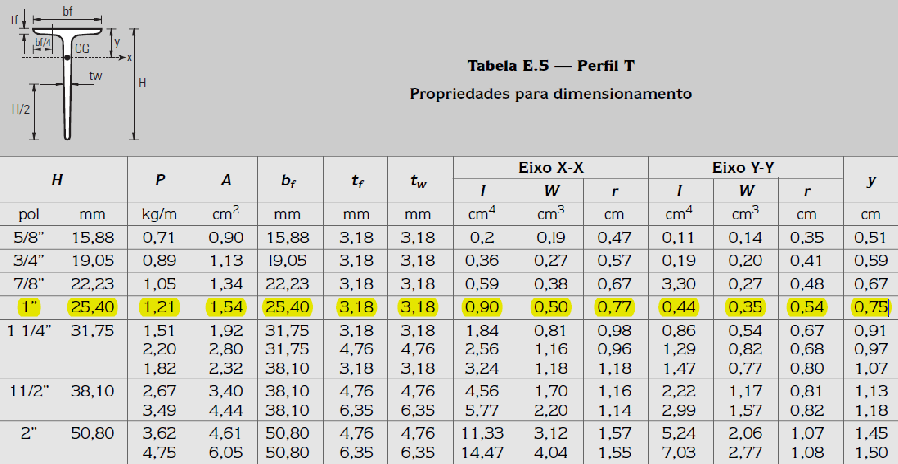
\includegraphics[scale=0.7]{figuras/perfil_t.png}
	\caption{Especificações do perfil em T}
\end{figure}

A resistência à flexão e da rigidez de flexão têm de ser calculado sobre um dos eixos, aquele que resultar no menor valor. Rigidez de flexão é proporcional ao produto EI e a resistência à flexão é dada pelo valor de é $\frac{S_{y}}{C}$ ( para o aço 1010 os valores são: $S_{y} = 370MPA$, E = 200...)

\begin{description}
	\item E Módulo de elasticidade;
	\item I Momento de inércia da secção transversal sobre o eixo com o menor valor
	\item $S_y$ Resistência ao escoamento do material em unidades de força por unidade de área;
	\item c Distância a partir do eixo neutro da fibra externa
\end{description}

\subsection{Teoria das Falhas}

A seguir, será explicitada a teoria das falhas. Pois a mesma será fundamental para a determinação de critérios que tem por objetivo, a previsão de falha em um determinado material sob tensão. Na seqüência serão apresentados os critérios mais clássicos para materiais dúcteis.

\subsubsection{Teoria da Tensão Máxima de Cisalhamento para Materiais Dúcteis}

Essa teoria se aplica somente a materiais dúctil, também conhecida como Teoria de Tresca ou de Guest. “Prevê que o escoamento começa sempre que a tensão máxima de cisalhamento em qualquer elemento iguala-se ou excede á tensão máxima de cisalhamento em uma espécime de ensaio de tração do mesmo material quando aquele espécime começa a escoar”. (SHIGLEY; MISCHKE, 2005)

Fortes teorias são criadas, baseando-se em testes de tração, onde as linhas de escoamento devem forma um ângulo de 45 graus com o eixo central do corpo de prova, como mostrado na figura X a seguir. Essas linhas concebem o início do escoamento, onde as linhas de fratura também são observadas a um ângulo de 45 graus.

\begin{figure}[h]
\centering
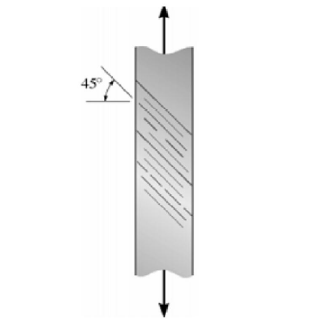
\includegraphics[scale=0.8]{figuras/linhas45.png}
\caption{Linhas de Lüder em uma tira de aço doce no seu escoamento (BEER FP E JOHNSTON,1995) }
\end{figure}

Para tensão de tração $\sigma = \frac{P}{A}$ onde a tensão máxima de cisalhamento é $\tau _{max} = \frac{\sigma}{2}$. Assumindo que $S_y$ é a resistência ao escoamento, no momento de escoamento, $\tau _{max} = \frac{S_{y}}{2}$ . Para um estado duplo de tensões, sabe-se que a máxima tensão de corte é:

\begin{equation}
\tau _{max} = \frac{\sigma_{1} - \sigma_{2}}{2}\leq \frac{S_{y}}{2}
\end{equation}

Onde: $\sigma_{1} \geq  \sigma_{2} \geq  \sigma_{3}$

Nesta teoria pode-se notar que a resistência ao escoamento em cisalhamento seja metade do limite de escoamento á tração:

\begin{equation}
S_{sy} = 0.5\times S_{y}
\end{equation}

Onde é necessário ainda, incorporar aos cálculos um fator de segurança n.

\begin{equation}
\tau_{max} \geq \frac{S_{y}}{2n}
\end{equation}

A figura \ref{teoria-tensao} a seguir, mostra o gráfico para a teoria da tensão máxima de cisalhamento em problemas biaxiais, onde uma das tensões principais é nula.

\begin{figure}[h]
\centering
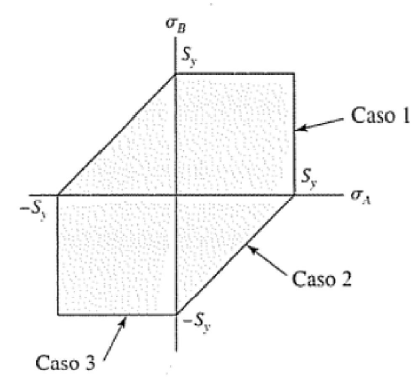
\includegraphics[scale=0.7]{figuras/tensao_cisa.png}
\caption{Teoria da tensão de cisalhamento máxima (MSS) para estado plano de tensão, sendo $\sigma_{A}$ e $\sigma_{B}$ as duas tensões principais não-nulas (BEER FP E  JOHNSTON,1995)}
\label{teoria-tensao}
\end{figure}

\subsubsection{Teoria da Energia de Distorção para Materiais Dúcteis}

Essa teoria é uma pouco mais difícil de ser empregada do que a teoria de tensão de cisalhamento máxima.

Também conhecido por teria da energia de cisalhamento e teoria de von-Mises-Hencky, originou-se quando foi observado que materiais dúcteis tensionados hidrostaticamente (tração ou compressão iguais) possuíam limite de escoamento muito maiores do que os valores dados pelo ensaio de tração simples. Huber-von Mises-Hencky postularam que o escoamento  não era um simples fenômeno de tração ou compressão, mais do que isso, era relacionado de algum modo a distorção angular do elemento tensionador.
A energia de distorção é obtida subtraindo da energia total de deformação a energia usada para provocar uma variação de volume. Onde para tensão plana, $\sigma_{A}$ e $\sigma_{B}$ as duas tensões principais não-nulas. Obtém-se:

\begin{equation}
{\sigma_{A}}' = \left ( \sigma^{2}_{A} - \sigma_{A}\sigma_{B}+\sigma^{2}_{B}\right )^{1/2} 
\end{equation}

A teoria de von-Mises prevê que a falha por escoamento ocorre sempre que:

\begin{equation}
{\sigma}' \geq S_{y}
\end{equation}

A figura \ref{energia-distorcao} mostra a elipse criada pela equação XY no plano $\sigma_{A}$, $\sigma_{B}$ com ${\sigma}' = S_{y}$. As linhas tracejadas apresentam a teoria da tensão máxima de cisalhamento, onde nos mostra um maior conservadorismo quando comparada com a teoria da energia de distorção.

\begin{figure}[h]
\centering
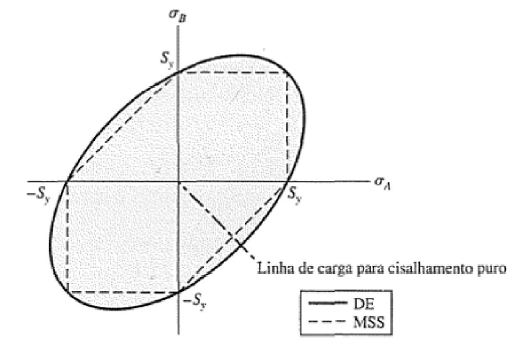
\includegraphics[scale=0.7]{figuras/teoria_distorc.png}
\caption{Teoria da energia de distorção (DE) para estados planos de tensão. Gráfico obtido com a partir da equação XY com  ${\sigma}' = S_{y}$ (BEER FP E JOHNSTON, 1995)}
\label{energia-distorcao}
\end{figure}

\subsubsection{Resumo das Falhas de Materiais Dúcteis}

Por conta do material usado na construção do suporte (tipo cavalete) para a bicicleta, ferro, que é dúctil, assim sendo será dado enfoque apenas a falhas em materiais dúcteis.

Joseph Marin (MARIN, 1952) foi um dos pioneiros no desenvolvimento de material relacionado à falha de elementos de engenharia. Alguns dos pontos abordados pelo autor que foram utilizados estão mostrados na figura \ref{teoria-falha} a seguir, onde alguns dos dados dispostos ao longo da linha inferior, onde se refere ao ferro fundido. A figura ainda mostra que tanto a teoria da tensão máxima de cisalhamento, quanto à energia de distorção são aceitáveis para projeto e análise de materiais que falham de forma dúctil.

A decisão quanto abordar um das duas teorias será explicitada mais adiante. A teoria da tensão máxima de cisalhamento é mais fácil, rápida de aplicar sendo mais conservadora. Caso se faz necessário descobrir por qual motivo alguma peça tenha falhado, então a teoria da energia de distorção é a mais aconselhada, devido às melhores aproximações com os dados coletados, mostrados no gráfico a seguir.

\begin{figure}[h]
\centering
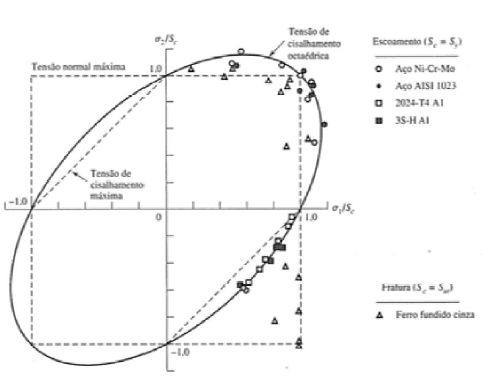
\includegraphics[scale=0.7]{figuras/falhas_norton.png}
\caption{Dados experimentais sobrepostos a teorias de falha (NORTON, 2000).}
\label{teoria-falha}
\end{figure}

\subsubsection{Introdução à Fadiga em Metais}

A maioria dos ensaios, a carga é aplicada gradualmente para que possa haver um tempo do desenvolvimento pleno da deformação. Os corpos de prova são ensaiados até sua plena destruição, sendo as tensões aplicadas somente uma vez. Esse tipo de ensaio é conhecido como condições estáticas as quais são bastante aplicáveis e se aproximam das condições em que máquinas, estruturas estão sujeitas. Normalmente surge outro tipo de carregamento, o qual passa de ser do gênero estático e viram tensões flutuantes ou variantes entre níveis. Um bom exemplo vem de eixos que sofrem rotação, os quais sofrem cargas de flexão, onde passam por etapas de compressão e tração ao longo de suas revoluções. Esses tipos de carregamentos produzem tensões chamadas de flutuantes, alternantes, repetidas ou variáveis.

Vários componentes falham devido a tensões repetidas, porém esse tipo de falha revela que as tensões reais estavam muito abaixo da resistência última do material até mesmo da resistência de escoamento. Daí vem à denominação de falha por fadiga. Fadiga é o processo progressivo e localizado de falha material, sob carregamento cíclico. Cerca de 80\% a 90\% das falhas que ocorrem em componentes e/ou estruturas são causadas por fadiga. Afeta, portanto, qualquer componente que se move e/ou que esteja sob solicitação cíclica, tais como automóveis nas estradas, aviões (principalmente as asas e a junção dessas com a fuselagem) em pleno vôo, pontos sob veículos, navios em alto mar, sob impacto das ondas (SANDOR, 1972)

Muitas falhas estáticas dão avisos visíveis antecipadamente, porém o mesmo não ocorre com a falha por fadiga, ela é súbita e sem aviso prévio, portanto perigosa. É um assunto mais complexo, onde projetar prevendo uma falha por fadiga é mais complexo e exige muito dos conhecimentos de um engenheiro. A aparência por falha por fadiga é muito semelhante a uma fratura frágil, apresentando superfícies de fratura planas e perpendiculares ao eixo da tensão.

De acordo com a teoria abordada por Norton (Norton, 2000), a falha por fadiga sempre inicia com uma fissura. A fissura pode estar presente no material devido ao processo de fabricação ou pode se desenvolver ao longo do tempo devido a uma deformação cíclica ao redor de regiões sujeitas a concentrações de tensões. As fissuras devido a fadiga geralmente iniciam em algum ponto onde há entalhes ou zonas de concentração de tensões. Conforme Norton (NORTON, 2000), há três estágios para a falha por fadiga:

\begin{enumerate}
	\item Início da trinca
	\item Propagação da trinca
	\item Fratura repentina
\end{enumerate}

Falha por fadiga se deve à formação de trinca e sua propagação. Essa trinca se iniciam, normalmente devida a uma descontinuidade no material. Vários fatores podem acelerar o início de trincas, onde, temperaturas elevadas, corrosão, ciclos de alta freqüência, ciclos de temperatura são fatores que afetam significativamente. A Figura \ref{parafuso-fadiga} mostra a superfície de uma falha por fadiga de um parafuso sob carregamento cíclico.

\begin{figure}[h]
\centering
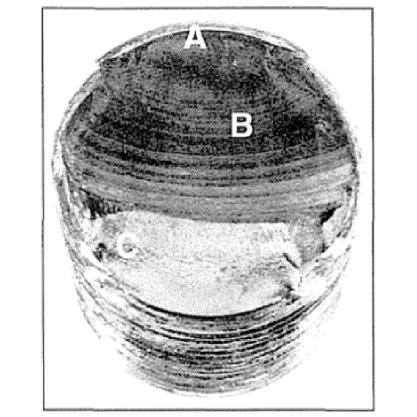
\includegraphics[scale=0.4]{figuras/parafuso_fadiga.jpg}
\caption{Falha por fadiga de um parafuso, em decorrência de flexão unidirecional repetida. A falha começou na raiz da rosca em A, propagou-se através da maior parte da secção transversal mostrada, como evidenciado pelas marcas de praia em B, antes da falha final em C.}
\label{parafuso-fadiga}
\end{figure}

\subsubsection{Abordagem da Falha por Fadiga em Análise e Projeto}

Toda e qualquer falha por fadiga, se inicia com uma pequena trinca, podendo estar presente desde sua manufatura até desenvolver ao longo do tempo. Sabendo que todo material possui descontinuidades, são três os estágios na falha por fadiga: início da trinca, propagação da trinca e fratura repentina.

\begin{itemize}
	\item Início da trinca: Não são trincas normalmente visíveis a olho nu. Tal início ocorre, por que os metais não são materiais homogêneos e isotrópicos os quais sofrem deformação plástica cíclica seguida de propagação cristalográfica estendendo-se por dois a cinco grãos, relativamente à origem.
	
	\item Propagação da trinca: Esse estágio se deve a tensões de  tração, onde a trinca se propaga ao longo de planos normais aos de tensão máxima de tração. Tensões cíclicas que são sempre de compressão não irão contribuir para o crescimento da trinca, onde sua tendência é fechá-la. Superfícies de fratura com platôs paralelos, separadas por sulcos também paralelos são formados, conhecidas como marcas 
	
	\item Fratura: A trinca continuará a crescer enquanto houver tensões de tração cíclica ou fatores de corrosão estiverem presentes. Em certo ponto, a trinca terá tamanho suficiente para que haja uma falha repentina, onde o fator de intensidade de tensão K e o nível da tenacidade à fratura do material $K_c$  tiverem aumento significativo.
\end{itemize}

Geralmente a ciência  não apresenta respostas completas que se fazem necessárias para solução do problema. Mas mesmo com esse impasse, onde a ciência não explica completamente o mecanismo de fadiga, o engenheiro deve continuar a projetar, peças ou estruturas que não irão falhar.

\subsubsection{Método da Vida sob Fadiga}

Existem três métodos de falhar por fadiga usados atualmente em projetos, são eles: método da vida sob tensão (S-N), método da vida sob deformação ($\in$-N) e o método da mecânica da fratura linear elástica (MFLE), cada um possuindo uma área de aplicação e um propósito. Neste trabalho  não será abordado o MFLE, devido a esse método necessitar que uma trinca já esteja presente e tenha sido detectada, sendo empregado para prever o crescimento dessa trinca.

\subsubsection{Método da Vida sob Tensão}

Várias técnicas foram elaboradas com propósito de medir e verificar respostas dos materiais submetidos a tensões deformações variantes no tempo. A mais antiga foi desenvolvida por Wohler que consistido por uma viga em balanço rotativa. R. R. Moore adaptou a técnica para eixos bi apoiados, essa máquinas realiza ensaios de flexão pura (sem cisalhamento transversal) por meio de pesos e é mais freqüentemente utilizada nas aplicações que envolvem fadiga de alto ciclo, nas quais espera-se que o conjunto mecânico opere por mais de 10\textsuperscript{3} ciclos de tensão aproximadamente.
 
	Diversos corpos de prova devem ser ensaiados para que possa estabelecer a resistência à fadiga de um material devido a sua natureza estática da fadiga. A carga aplicada é decrescente, sendo o primeiro ensaio realizado com uma tensão um pouco inferior á resistência última do material. O segundo é feito com uma tensão menor que a anterior e assim sucessivamente onde é traçado um diagrama S-N na figura \ref{wohler}. A ordenada do diagrama S-N é denominada resistência à fadiga $S_f$ e a abscissa é referente ao número de ciclos N correspondente a essa resistência.
	
\begin{figure}[h]
\centering
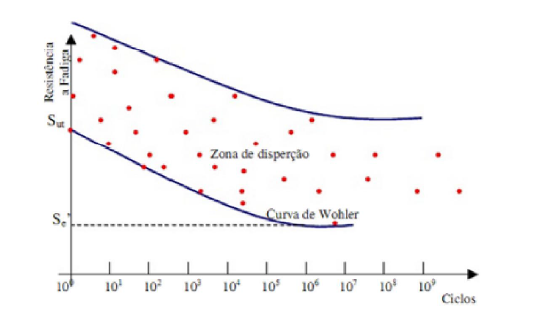
\includegraphics[scale=0.8]{figuras/wohler.png}
\caption{Curva de Wohler.}
\label{wohler}
\end{figure}

Ao elevar os valores obtidos na curva de Wohler para um gráfico com coordenadas logarítmicas como na figura \ref{fadiga-axial}, percebe-se que o número de ciclos necessários para provocar a ruptura aumenta rapidamente com o decréscimo da carga aplicada. Esse gráfico determina que para certa carga a vida da peça é infinita, independente do número de ciclos. Essa inflexão (“joelho”) define o limite de fadiga $S_e$, para o material ensaiado.

\begin{figure}[h]
\centering
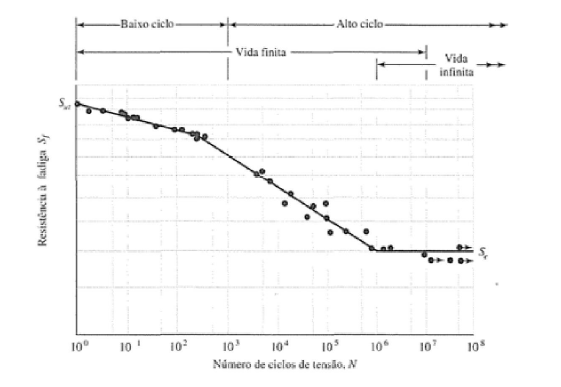
\includegraphics[scale=0.8]{figuras/num_ciclos.png}
\caption{Um diagrama S-N traçado a partir dos resultados de testes de fadiga axial completamente inversa. Material: aço UNSG 41300.}
\label{fadiga-axial}
\end{figure}

Esse método é o menos preciso para aplicações de baixa ciclagem. Porém é o método mais tradicional, apresentando muitos dados publicados. É o de mais fácil implementação para muitas aplicações de projeto e apresenta adequadamente aplicações de alta ciclagem.

\subsubsection{Método da Vida sob Deformação}

Esse método é aplicado com maior freqüência em regimes de fadiga de baixo ciclo e em problemas de vida finita, nos quais as tensões cíclicas são elevadas o suficiente para causarem escoamento local. É o melhor método já apresentado para explicar a natureza da falha por fadiga (Shigley).

	Geralmente uma falha por fadiga tem como início uma descontinuidade local, tal como um entalhe, uma trinca ou outra área de concentração de tensão (Shigley). Devido ao fato de a iniciação de uma trinca envolver escoamento, modelos que usam aproximações que se baseiam na tensão são incapazes de fazer uma modelagem adequada para esse estágio de fadiga. Se uma fratura por fadiga está para ocorrer, deve haver deformações plásticas (Shigley).
	
	Os limites elásticos do ferro e do aço podem ser mudados – para mais ou para menos – por variações cíclicas de tensão. Em geral, os limites elásticos de aço recozido devem provavelmente aumentar quando sujeitos a ciclos de inversão de tensão, ao passo que aços repuxados a frio exibem um limite elástico decrescente (Shigley).

	A figura \ref{histerese}, foi construída com o fim de mostrar a aparência geral de gráficos de tensão-deformação cíclica para uma grande quantidade de aços de resistência muito alta para os primeiros poucos ciclos de deformação cíclica controlada.

\begin{figure}[h]
\centering
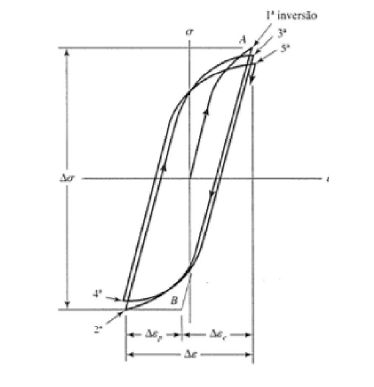
\includegraphics[scale=0.8]{figuras/histerese.png}
\caption{Os ciclos de histerese da tensão verdadeira-deformação, mostrando as primeiras cinco versões de tensão de um material com amolecimento cíclico.}
\label{histerese}
\end{figure}

\subsubsection{Limite de resistência}

nsaios de fadiga são muitos usados para a determinação dos limites de resistência porém é um processo bastante longo, onde ensaios de tensão são preferidos quando comparados aos de deformação.
	A figura \ref{grafico-limites}, mostra uma relação entre dois conjuntos de dados retirados de ensaios com vigas rotativas e ensaios de tração simples. Isso é feito pois para uma análise preliminar, um método rápido de estimativa dos limites de resistência é necessário. O gráfico parece sugerir que o limite de resistência Vaira entre cerca de 40\% a 60\% da resistência à tração para aços de até 212 kpis (1460 Mpa) aproximadamente (Shigley).
	
\begin{figure}[h]
\centering
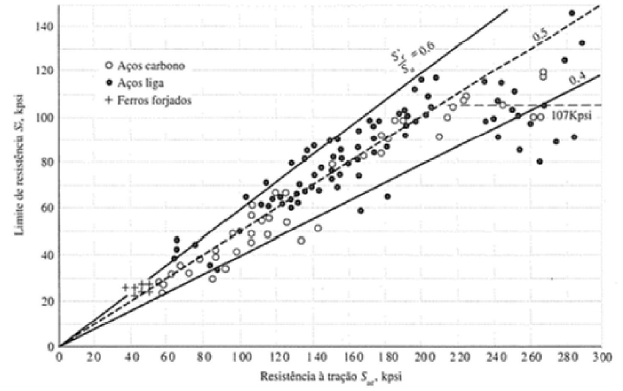
\includegraphics[scale=0.6]{figuras/resistencia_tracao.png}
\caption{Gráfico dos limites de resistência versus resistência à tração procedente de resultados de ensaios verdadeiros para uma grande quantidade de ferros forjados e de aços.}
\label{grafico-limites}
\end{figure}

Estimativas obtidas de dados de uma série de fontes podem apresentar uma grande variação em seus resultados, podendo desviar significativamente dos resultados reais obtidos em laboratório. Sendo a área de incerteza grande, uma compensação maior que aquelas utilizadas em projeto estático devem ser empregadas.

\subsection{Simulação Numérica}

Uma vez construída a base em treliça, fez-se necessário a aplicações de esforços os quais a mesma será solicita, assim que o usuário se sentar na bicicleta. Porém, para início de dados gerados, foi feita uma análise sobre as distribuições de esforços sobre a bicicleta, uma vez que mesma estiva apoiada, apenas através do ‘garfo’ que serve para ligar o quadro, a roda, como pode ser visto na figura \ref{pontos-esforcos}:

\begin{figure}[h]
\centering
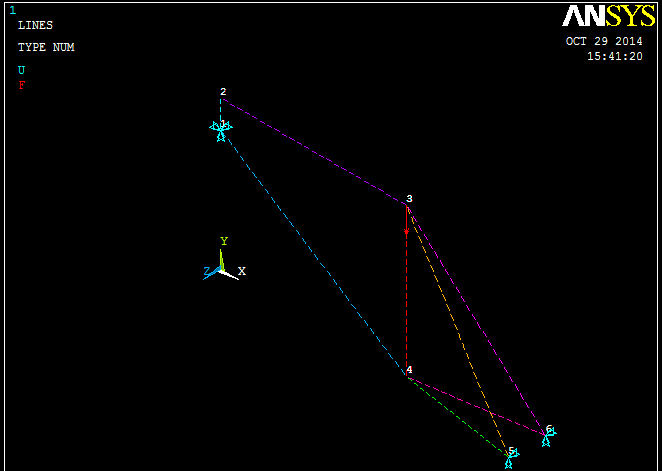
\includegraphics[scale=0.5]{figuras/3D_bike.png}
\caption{Pontos de esforços.}
\label{pontos-esforcos}
\end{figure}

Onde, na sete em vermelho foi aplicada a carga gerada pelo ciclista, um valor igual a no máximo 1.000N. Os pontos 1, 5 e 6 foram usados para fixar a bicicleta, e analisar as reações nos mesmos, pois, o suporte será fixo nos pontos 1, 5 6.

Utilizando-se o software \textit{ansys}, foi feita uma simulação, adotando as característica da uma bicicleta que será utilizada pelo usuário, do tipo aro 26, feita em alumínio, com um perfil circular vazado de diâmetro externo igual a 25mm com 2mm de espessura.

\begin{figure}[h]
\centering
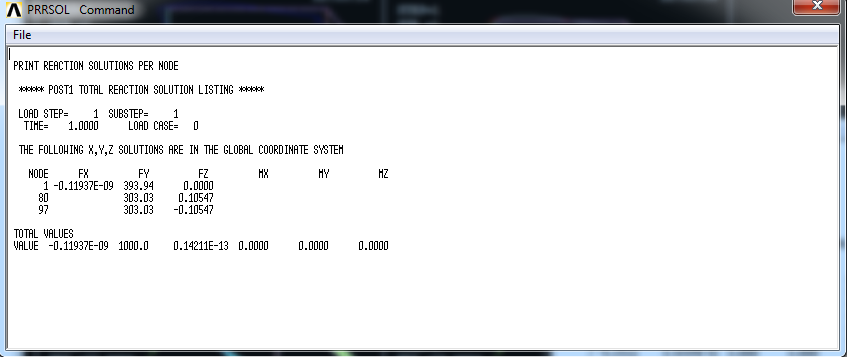
\includegraphics[scale=0.5]{figuras/reacoes.png}
\caption{Simulação}
\end{figure}

Onde, em 1 temos uma carga igual a 393,94N e em 5 e 6, uma carga igual a 303,03N. Usando estes valores encontrados no Ansys, através da simulação em 3D da bicicleta, foi feita uma simulação usando o CATIA VR19,no suporte já desenhado, para verificar se o suporte projetado, consegue suportar as solicitações impostas. Como temos na figura \ref{resultado-simulacao} e \ref{analise-deslocamento}.

\begin{figure}[h]
\centering
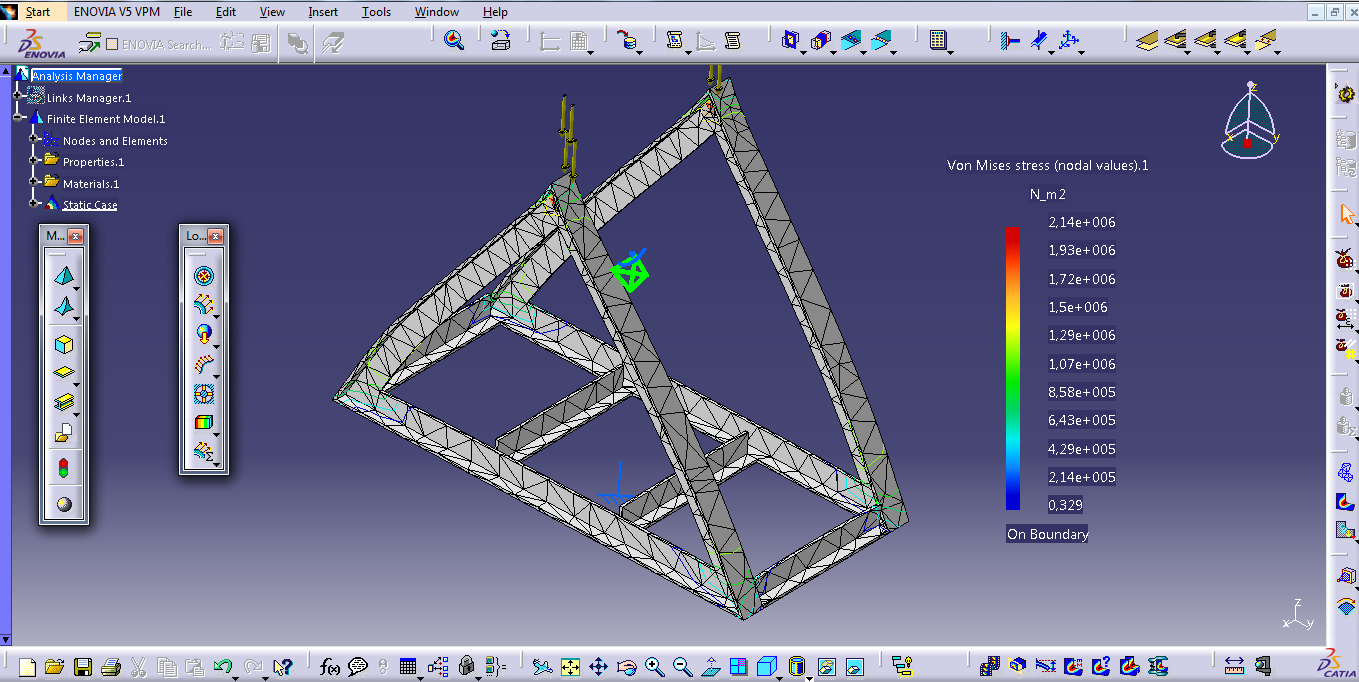
\includegraphics[scale=0.4]{figuras/vonmisses.png}
\caption{O resultado para a análise de Von Misses}
\label{resultado-simulacao}
\end{figure}

\begin{figure}[h]
\centering
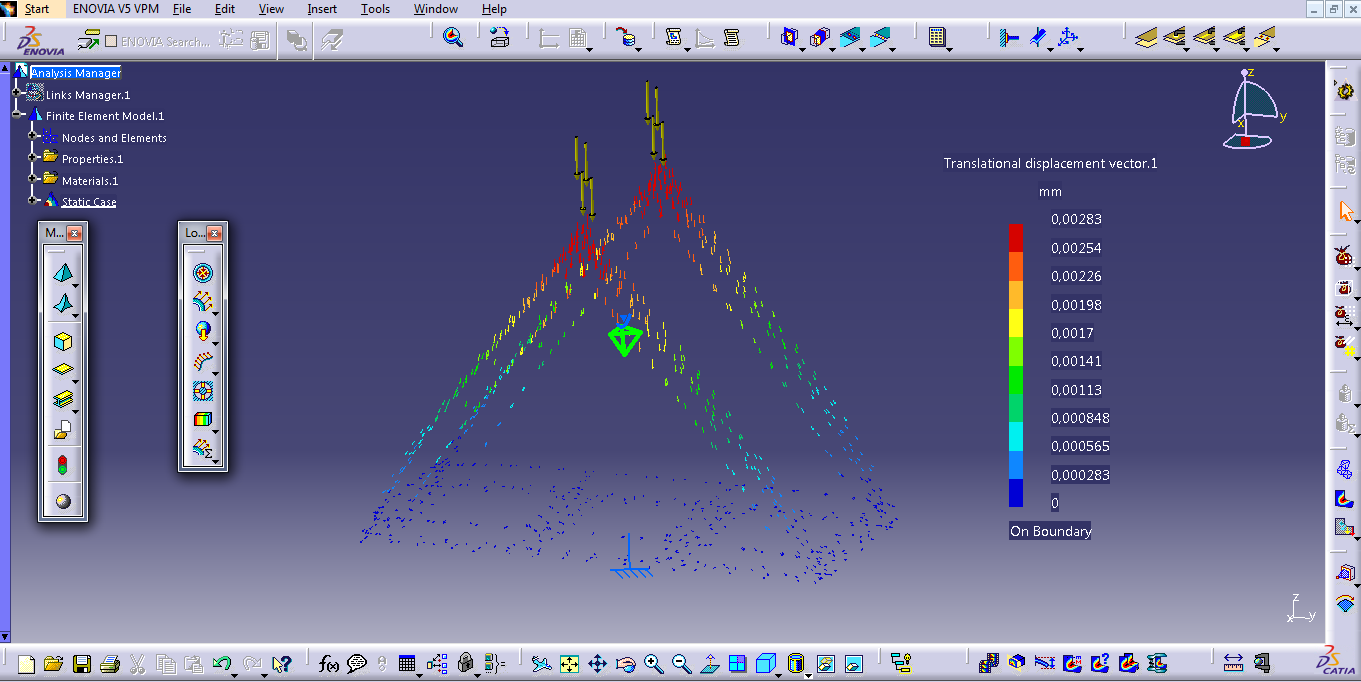
\includegraphics[scale=0.4]{figuras/deslocamento.png}
\caption{O resultado para a análise de deslocamento.}
\label{analise-deslocamento}
\end{figure}
